\documentclass[border=6pt]{standalone}
\usepackage{tikz}
\usetikzlibrary{arrows.meta,positioning,calc,shapes.geometric,fit,backgrounds,patterns,matrix,decorations.pathreplacing}
\begin{document}
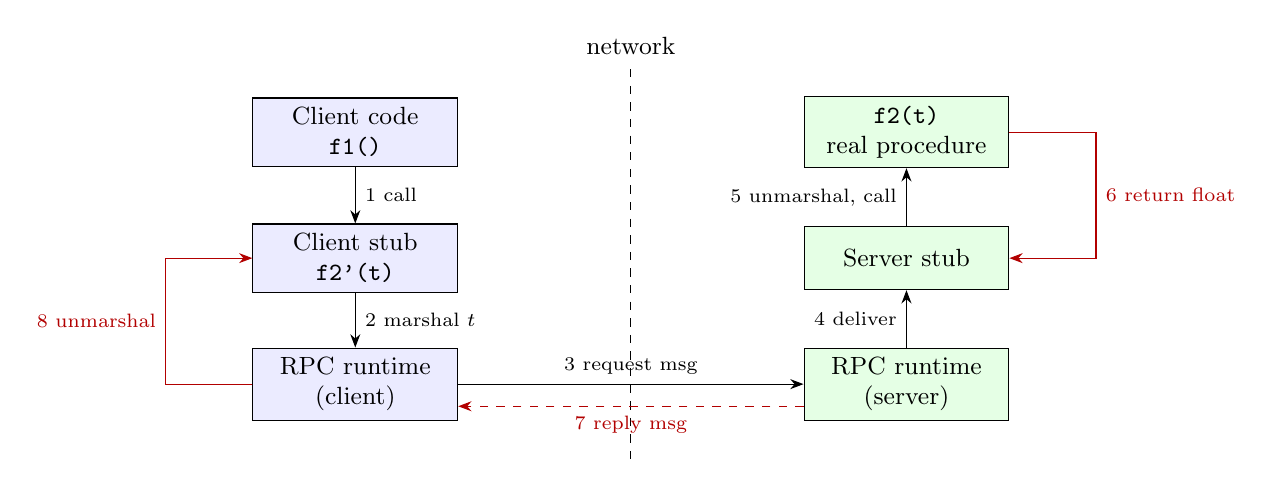
\begin{tikzpicture}[>=Stealth,font=\small]
\tikzstyle{box}=[draw,minimum width=2.6cm,minimum height=0.8cm,fill=blue!8,align=center]
\node[box] (f1) at (0,0) {Client code\\ \texttt{f1()}};
\node[box] (cs) at (0,-1.6) {Client stub\\ \texttt{f2'(t)}};
\node[box] (cr) at (0,-3.2) {RPC runtime\\ (client)};
\node[box,fill=green!10] (sr) at (7,-3.2) {RPC runtime\\ (server)};
\node[box,fill=green!10] (ss) at (7,-1.6) {Server stub};
\node[box,fill=green!10] (f2) at (7,0) {\texttt{f2(t)}\\ real procedure};
\draw[dashed] (3.5,0.8) -- (3.5,-4.2); \node at (3.5,1.1) {network};
\draw[->] (f1) -- node[right,font=\scriptsize]{1 call} (cs);
\draw[->] (cs) -- node[right,font=\scriptsize]{2 marshal $t$} (cr);
\draw[->] (cr) -- node[above,font=\scriptsize]{3 request msg} (sr);
\draw[->] (sr) -- node[left,font=\scriptsize]{4 deliver} (ss);
\draw[->] (ss) -- node[left,font=\scriptsize]{5 unmarshal,\ call} (f2);
\draw[->,red!70!black] (f2.east) -- ++(1.1,0) |- node[pos=0.25,right,font=\scriptsize]{6 return float} (ss.east);
\draw[->,red!70!black,dashed] ([yshift=-8pt]sr.west) -- node[below,font=\scriptsize]{7 reply msg} ([yshift=-8pt]cr.east);
\draw[->,red!70!black] (cr.west) -- ++(-1.1,0) |- node[pos=0.25,left,font=\scriptsize]{8 unmarshal} (cs.west);
\end{tikzpicture}
\end{document}
